\documentclass[tikz,border=8pt]{standalone}
\usepackage{pgfplots}
\usepgfplotslibrary{groupplots}
\pgfplotsset{compat=1.18}
\begin{document}
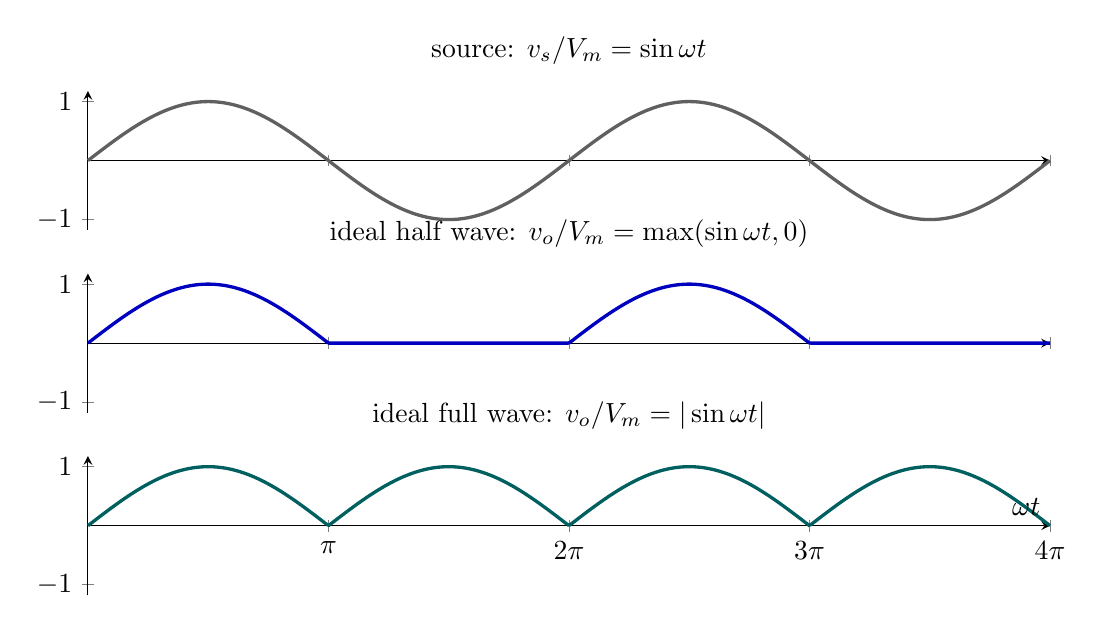
\begin{tikzpicture}
\begin{groupplot}[
  group style={group size=1 by 3,vertical sep=0.55cm},
  width=13.8cm,height=3.35cm,
  xmin=0,xmax=12.5664,ymin=-1.18,ymax=1.18,
  axis lines=middle,
  xtick={0,3.1416,6.2832,9.4248,12.5664},
  xticklabels={$0$,$\pi$,$2\pi$,$3\pi$,$4\pi$},
  ytick={-1,0,1},clip=false
]
\nextgroupplot[title={source: $v_s/V_m=\sin\omega t$},xticklabels={}]
\addplot[very thick,gray!75!black,domain=0:12.5664,samples=500]{sin(deg(x))};
\nextgroupplot[title={ideal half wave: $v_o/V_m=\max(\sin\omega t,0)$},xticklabels={}]
\addplot[very thick,blue!75!black,domain=0:12.5664,samples=500]{max(sin(deg(x)),0)};
\nextgroupplot[title={ideal full wave: $v_o/V_m=|\sin\omega t|$},xlabel={$\omega t$}]
\addplot[very thick,teal!75!black,domain=0:12.5664,samples=500]{abs(sin(deg(x)))};
\end{groupplot}
\end{tikzpicture}
\end{document}
